% Copyright (C) The IMR developers. SPDX-License-Identifier: GPL-3.0-or-later
\documentclass[tikz,border=8pt]{standalone}
\usepackage[T1]{fontenc}
\usepackage{lmodern}
\usetikzlibrary{arrows.meta}
\definecolor{ink}{HTML}{122D4A}
\definecolor{wave}{HTML}{2776C9}
\definecolor{heat}{HTML}{DF8D32}
\definecolor{rheo}{HTML}{168B88}
\begin{document}
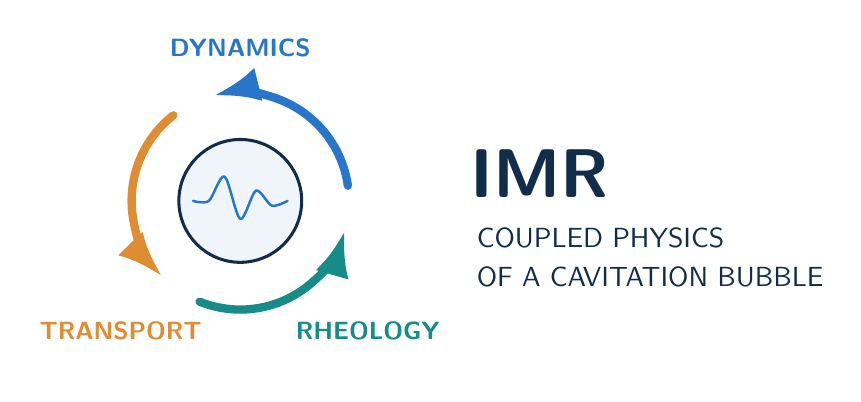
\begin{tikzpicture}[>=Latex,font=\sffamily,line cap=round,line join=round]
  \fill[white] (-2.7,-2.2) rectangle (7.5,2.2);
  \foreach \start/\col in {8/wave,128/heat,248/rheo} {
    \draw[->,\col,line width=3pt] (\start:1.38) arc[start angle=\start,end angle=\start+96,radius=1.38];
  }
  \fill[wave!7] (0,0) circle (.78);
  \draw[ink,line width=1.1pt] (0,0) circle (.78);
  \draw[wave,line width=.9pt] plot[smooth] coordinates {(-.6,0) (-.4,0) (-.2,.31) (0,-.23) (.2,.13) (.4,-.06) (.6,0)};
  \node[text=wave,font=\sffamily\bfseries\small] at (0,1.95) {DYNAMICS};
  \node[text=heat,font=\sffamily\bfseries\small] at (-1.52,-1.65) {TRANSPORT};
  \node[text=rheo,font=\sffamily\bfseries\small] at (1.62,-1.65) {RHEOLOGY};
  \node[anchor=west,text=ink,font=\sffamily\bfseries\fontsize{49}{52}\selectfont] at (2.8,.35) {IMR};
  \node[anchor=west,text=ink,font=\sffamily\fontsize{10}{14}\selectfont,align=left] at (2.88,-.72)
    {COUPLED PHYSICS\\OF A CAVITATION BUBBLE};
\end{tikzpicture}
\end{document}
